\documentclass{beamer}

% importations de packages utiles
\usepackage[utf8]{inputenc}  % pouvoir écrire avec des accents
\usepackage[french]{babel}  % francophopnie
\usepackage{amsmath}
\usepackage{array}
\usepackage{hyperref}  % liens clicables dans pdf final
\usepackage{tikz}  % pouvoir tracer des dessins sympas
\usetikzlibrary{calc}  % pour subtilités dans l'étiquettage d'images
\usetheme{Boadilla}  % thème de beamer
\usepackage{listingsutf8}  % rendu de "code" (avec config ci-dessous)
% configuration de lstlisting pour montrer du code python
\definecolor{lstcolor}{rgb}{0.9,0.95,0.95}
\definecolor{lstcommentcolor}{rgb}{0.,0.2,0.}
\lstset{
  frameround=tttt,
  %autogobble,
  frame=single,
  backgroundcolor=\color{lstcolor},
  % extendedchars=true,
  % basicstyle=\ttfamily\small,
  keywordstyle=\bfseries\color{blue},
  identifierstyle=\bfseries\color{red},
  stringstyle=\bfseries\color{orange},
  commentstyle=\color{lstcommentcolor},
  language=Python,
  keepspaces=True,
  basicstyle=\fontfamily{pcr}\selectfont\small, % monospace it for copypasting
  upquote=true,
  columns=flexible,
  showstringspaces=False,
  literate={é}{{\'e}}1
}

% table des matières locale
\newcommand\minitoc{
  \begin{frame}{\secname}
    \tableofcontents[currentsection, hideothersubsections, ] %  sectionstyle=show/show]
  \end{frame}
}
\newcommand\subminitoc{
  \begin{frame}{\subsecname}
    \tableofcontents[currentsubsection, hideothersubsections,
    sectionstyle=show/shaded, subsectionstyle=show/hide, subsubsectionstyle=show/hide]
  \end{frame}
}

% ignorer toute une section sans utiliser des % de commentaire
\newcommand\ignore[1]{}

% options pour la page de titre
\title{Projet \textit{RNG}}
\subtitle{Algorithmes et Structures de Données II} \author{Juan-Carlos Barros,
  Yves Dethurens,\\ Daniel Kessler et Jean-Francis Ravoux}

% et c'est parti
\begin{document}
\begin{frame}
  \titlepage
  \begin{center}
    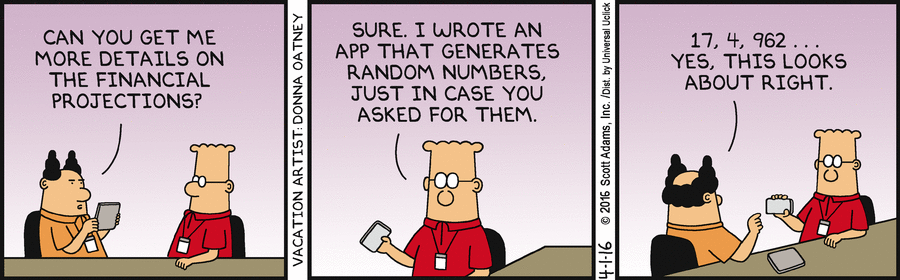
\includegraphics[width=.8\textwidth]{img/dilbert_financial.png}    
  \end{center}
\end{frame} % titre
\author{JCB, YD, DK, JFR}

\section{Introduction}
\minitoc
\subsection{À quoi servent les RNG?}
\begin{frame}{À quoi servent les Générateurs de Nombres Aléatoires?}
  \begin{center}
   
\includegraphics[width=.3\textwidth]{img/rng_calm.png}
  % \includegraphics<2->[width=.4\textwidth]{img/rng_skill.png}
  %\par\medskip
  %\includegraphics<3->[width=.8\textwidth]{img/dilbert_financial.png}
  \end{center}
  \end{frame}

\ignore{
\subsection{Que veut-on simuler?}
\begin{frame}{Que veut-on simuler?}
  \begin{itemize}
  \item Des $001101001\ldots$ aléatoires de la taille d'un \textbf{mot machine}\medskip
  \item<2-> Des nombres entre 0 et $2^{32} - 1$ ``tirés au hasard''
    \medskip
  \item<3-> Des nombres entre 0 et 1 \textbf{uniformément distribués}
  \end{itemize}
\end{frame}
}

\subsection{Vrai ou pseudo aléatoire?}
\begin{frame}
  \frametitle{Vrai ou pseudo aléatoire?}
  \begin{itemize}
  \item<1-> À partir de données ``physiques'' (TRNG)
    \begin{center}
      \begin{tabular}{>{\centering}m{.3\textwidth}>{\centering}m{.4\textwidth}}
      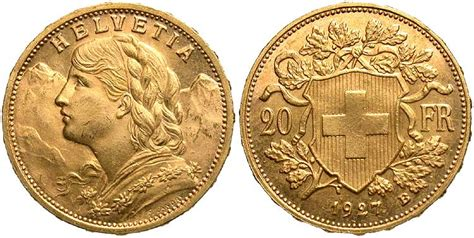
\includegraphics[width=.2\textwidth]{img/vreneli.png}&
      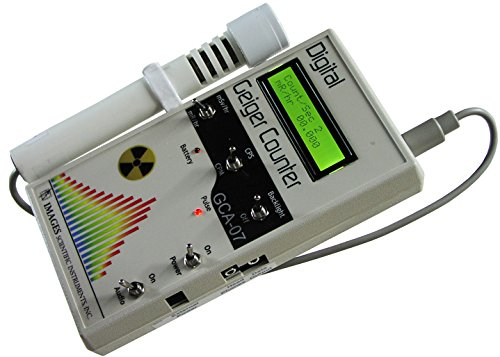
\includegraphics[width=.3\textwidth]{img/geiger.png}        
      \end{tabular}
    \end{center}
  \item<2-> Avec un algorithme déterministe (PRNG)
  \begin{center}
%    \begin{minipage}{0.33\textwidth}
%    \includegraphics<1->[width=.7\textwidth]{img/xkcd_sports.png}
%    \end{minipage}
    \begin{minipage}{0.65\textwidth}
    \includegraphics<2->[width=.8\textwidth]{img/xkcd_fair.png}
    \end{minipage}
    \par
    \onslide<2->{(source: xkcd.com)}
  \end{center}
  \end{itemize}
\end{frame}

\ignore{
  \section{Générateurs de nombres pseudo-aléatoires}
  \minitoc
}
\subsection{Caractéristiques communes des PRNG}
\begin{frame}{Générateurs de nombres pseudo-aléatoires}
  \only<1->{
    Exemple de générateur heuristique ``naïf'' (utilisé aux années 1950):

    \[30472901 \overset{\text{carré}}\longrightarrow
      {\color<2->{blue}0928}59769535{\color<2->{blue}5801}
      \onslide<3->{\overset{\text{tronqué}}\longrightarrow 59769535}\]
    
  }
  \onslide<4->{
  Les Pseudo Random Number Generators (PRNG) génèrent:
  \begin{itemize}
  \item une \textbf{suite} de nombres de manière \textbf{déterministe} (et
    ``sans histoire'')
  \item<5-> à partir d'une \textbf{seed} (nombre initial)
  \item<6-> avec une certaine \textbf{période}\par
    (a priori limitée à $2^{32}$ pour des nombres à 32 bits, par exemple)
  \end{itemize}
  }
\end{frame}

\ignore{
\subsection{Générateurs à congruence linéaire (LCG)}
\begin{frame}{Générateurs à congruence linéaire (LCG)}
  Pour l'instant ceci est un exemple de mise en page pour JF
  \begin{minipage}{0.32\textwidth}
    \onslide<1->{Du texte inutile gauche\par}
    \onslide<2->{Du texte inutile en plus}
  \end{minipage}
  \begin{minipage}{0.33\textwidth}
    Du texte inutile central
  \end{minipage}
  \begin{minipage}{0.32\textwidth}
    \only<1-2>{Du texte inutile droit}
    \only<3->{Un texte différent}
  \end{minipage}
\end{frame}
}
\section{Générateurs à Congruence Linéaire (LCG)}
\minitoc
\subsection{Explication de l'algorithme}
\begin{frame}{Générateurs à Congruence Linéaire (LCG)}
  \begin{minipage}{\textwidth}
    \only<1,4,5>{\begin{figure}
      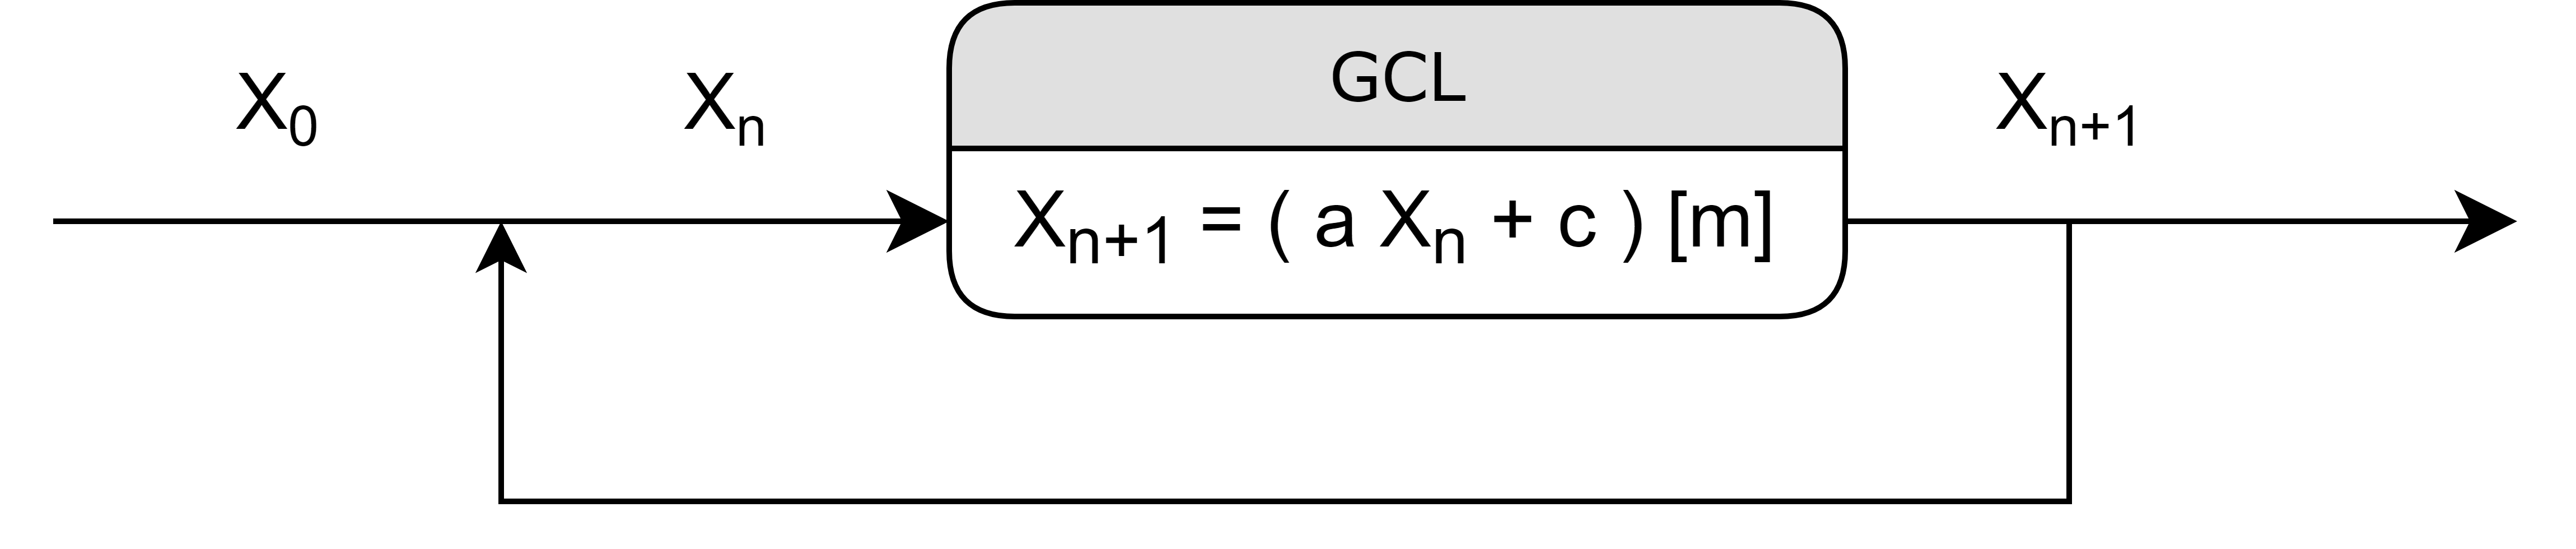
\includegraphics[scale=1]{img/GCL1-général.png}
      \end{figure}\par}
    \only<2>{\begin{figure}
      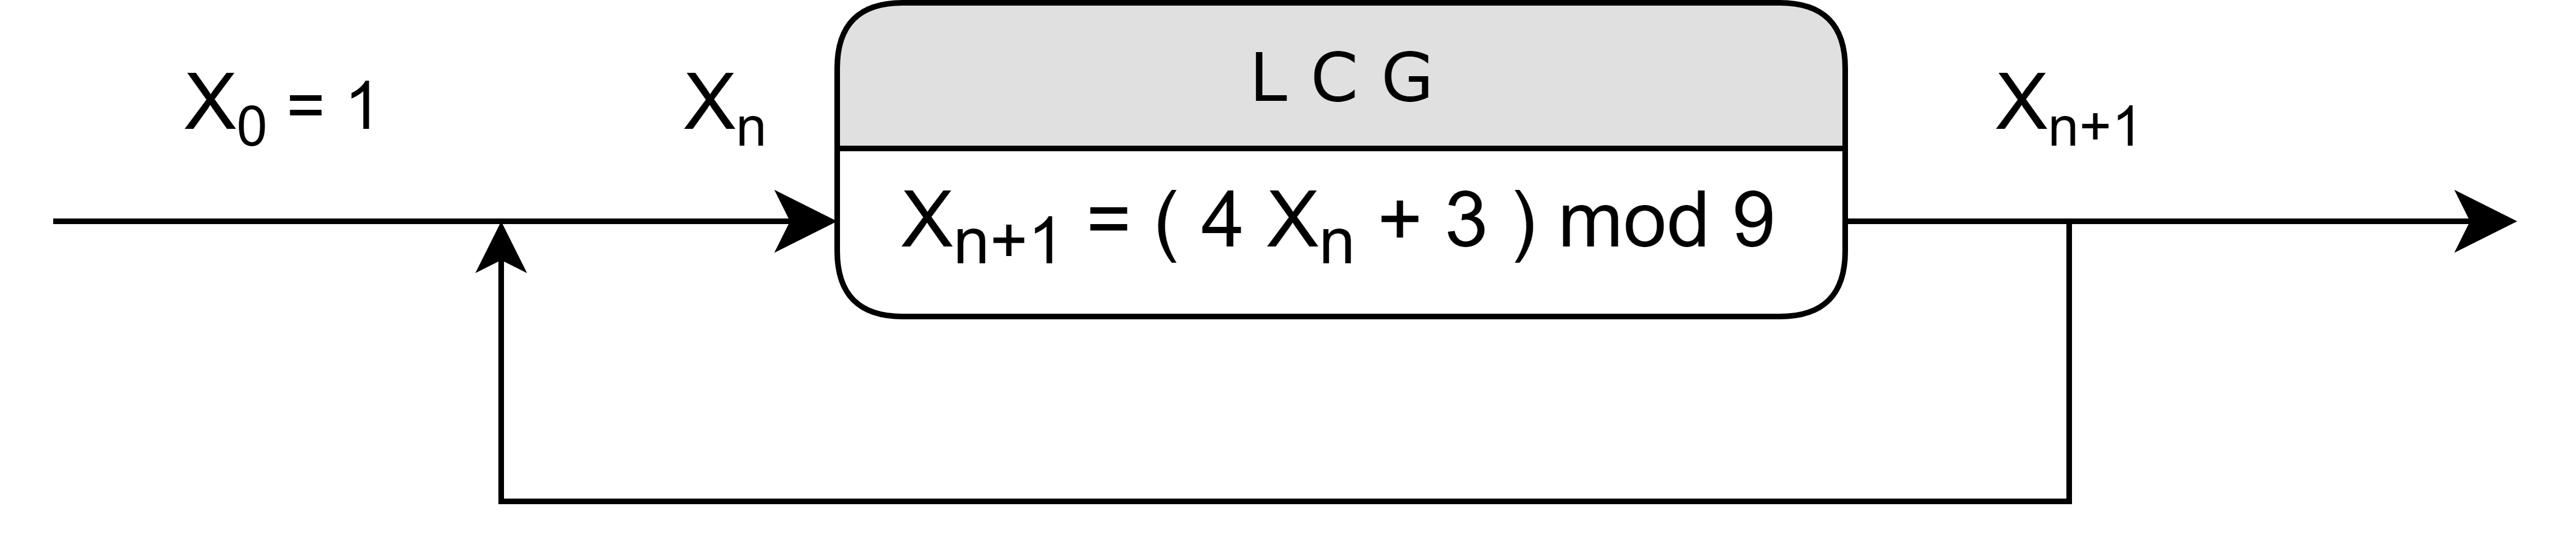
\includegraphics[scale=1]{img/GCL1-val1.png}
      \end{figure}\par}
    \only<3>{\begin{figure}
      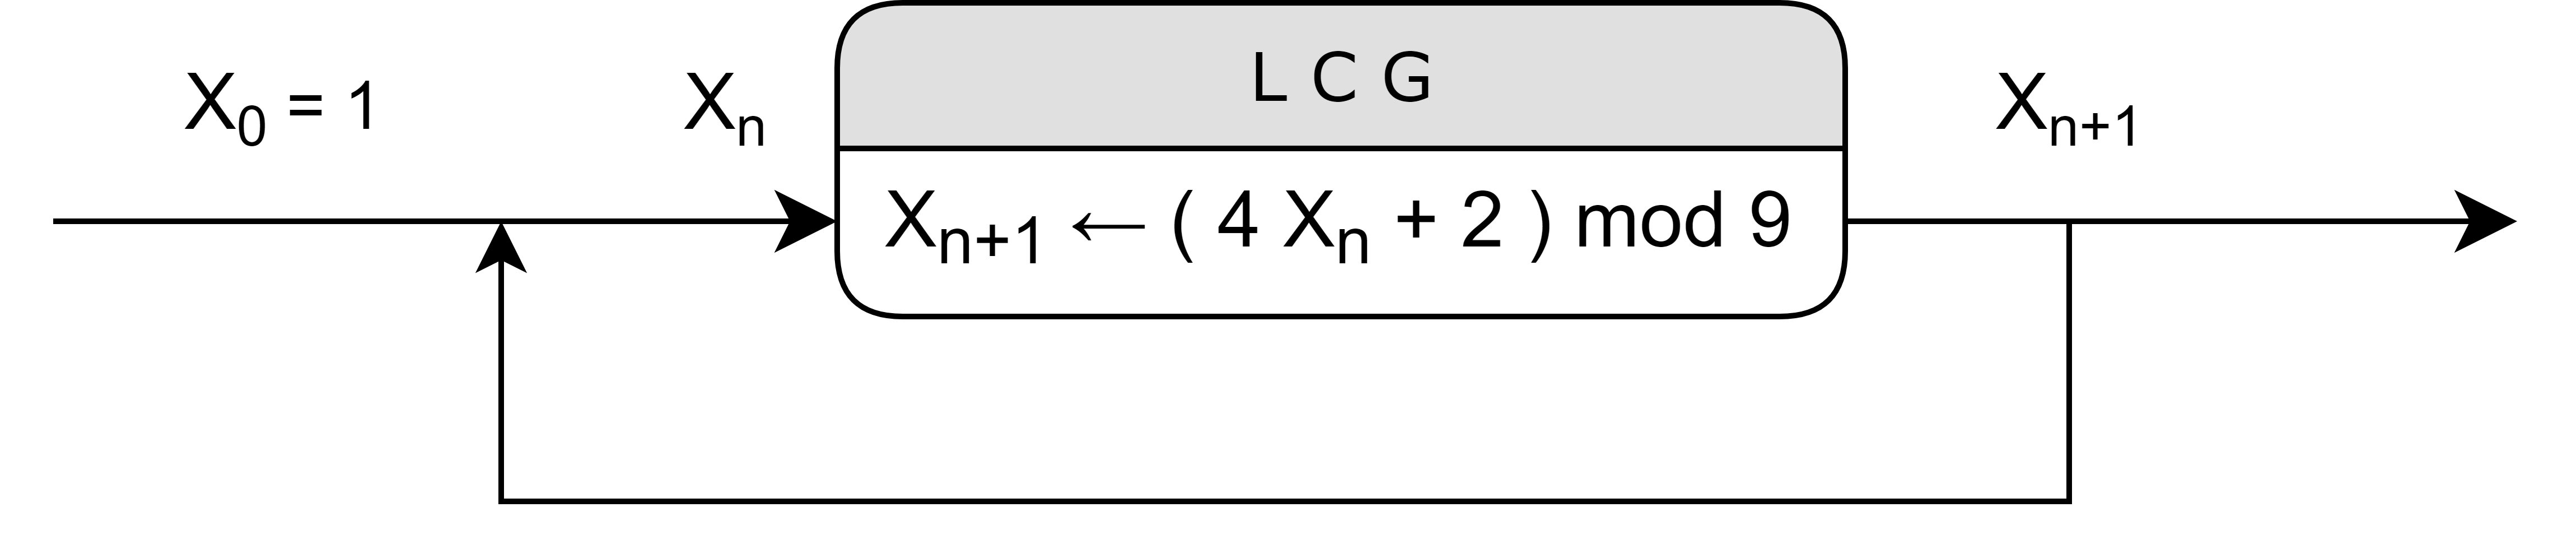
\includegraphics[scale=1]{img/GCL1-val2-magic.png}
      \end{figure}\par}
  \end{minipage}

  \begin{minipage}{0.27\textwidth}
    \onslide<1->{$m$ module \\
    $a$ multiplicateur \\
    $c$ incrément \\
    $X_0$ graine \\
    $X_{n} \in \{0, .., m-1\}$\par}
  \end{minipage}
  % \begin{minipage}{0.33\textwidth}
  %   Du texte inutile
  % \end{minipage}
  \begin{minipage}{0.72\textwidth}
    \only<2>{Cas 1: $X_n = 1,0,2,3,1,\ldots$ \\ période $p = 4$}
    \only<3>{Cas 2: $X_n = 4,0,2,1,6,8,7,3,5,4,\ldots$\\ période $p = 9$}
    \only<4>{Cas 1: ($a=3$,
      $c=2$, $m=5$) mauvaises valeurs \par
      Cas 2: ($a=4$, $c=2$, $m=9$) valeurs magiques\par
      conditions pour optimiser les nombres aléatoires:\par
      module grand\par
      conditions sur $a$ et $c$ pour maximiser $p$ }
    % \only<5>{Critères:\\
    % PGCD(a,m)=1;PGCD(c,m)=1\\
    % m multiple d'un nombre premier alors a-1 est multiple de ce nombre\\
    % a-1 est multiple de 4 si m est multiple de 4 }
    \only<5>{\hspace{-1em}\small
    \begin{tabular}{rl}
      IBM& $X_{n+1} \leftarrow (65539 X_{n}) \mod 2^{31}$\\
      Turbo Pascal& $X_{n+1} \leftarrow (129 X_{n} + 907633385) \mod 2^{32}$\\
      Unix& $X_{n+1} \leftarrow (1103515245 X_{n}+12345) \mod 2^{31}$
    \end{tabular}
}
  \end{minipage}
\end{frame}
\subsection{Suite aléatoire? (tests)}
\begin{frame}{LCG: Suite aléatoire?}
  Exemples de tests spectraux pour 100 nombres successifs
    \begin{figure}
      \begin{center}
      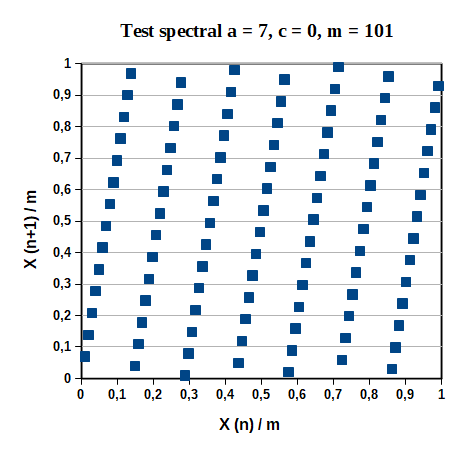
\includegraphics[scale=0.4]{img/a7m101.png}
      \hspace{0.1\textwidth}
      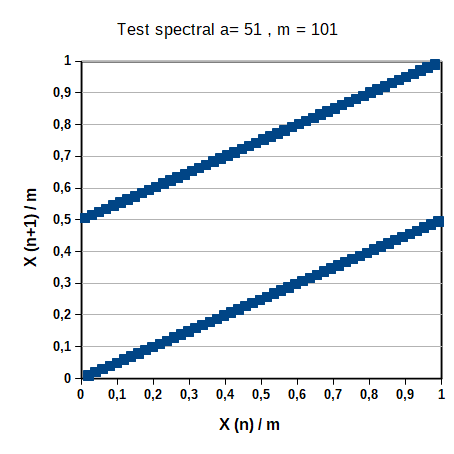
\includegraphics[scale=0.4]{img/a51m101.png}
      \end{center}
    \end{figure}
    % discrépance : mesure de l'homogénéité et du recouvrement\par
    % faible $\rightarrow$ couverture fine et homogène des nombres générés dans $[0,1]^2$
\end{frame}

\section{Vrai chaos déterministe}
\minitoc
\ignore{
\begin{frame}
  \frametitle{Vrai chaos déterministe}
  \begin{itemize}
  \item générateurs basés sur la \textbf{théorie des nombres}
    \begin{itemize}
    \item suites périodiques
    \item suites prévisibles
    \end{itemize}
  \item

  \item<2->
    générateurs basés sur la \textbf{théorie du chaos}
    \begin{itemize}
    \item suites imprévisibles
    \item ...mais peut-être périodiques!
    \end{itemize}  
  \item

  \item<3-> le générateur pseudo-aléatoire de Saito \&
    Yamaguchi (2017) utilise les deux théories
  \end{itemize}   
\end{frame}
}
\subsection{Décalage de Bernouilli}
\begin{frame}
  \frametitle{Point de départ : décalage de Bernoulli}
  \begin{center}
    {\LARGE $\alpha_{n+1} \leftarrow (2\alpha_n)\mod1$\par}
    \medskip
    définit une suite où $\alpha_n \in [0;1[$.
  \end{center}
  \onslide<2->{
    \par
    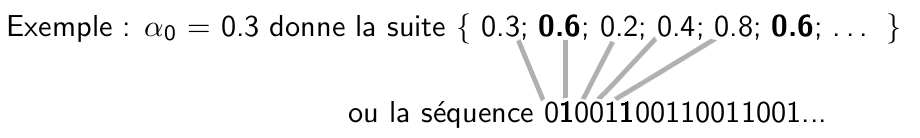
\includegraphics[scale=1]{img/correspondance.png}}
  \medskip
  \onslide<3->
  \begin{itemize}
  \item<3-> si $\alpha_0$ est \textbf{rationnel} $\Rightarrow$ suite périodique, très prévisible \\
  \item<4-> si $\alpha_0$ est \textbf{irrationnel} $\Rightarrow$ suite \textbf{non périodique}
  \end{itemize}
  \onslide<5->{
    \medskip
    Variation infinitésimale de $\alpha_0 \Rightarrow$ changement radical de la suite \\}
  \onslide<6->{
    \begin{center}
      sensibilité aux conditions initiales :\\
      caractéristique d'un processus \textbf{chaotique}
    \end{center}}
\end{frame}
\subsection{Sensibilité aux conditions initiales}
\begin{frame}
  \definecolor{bleu}{rgb}{0.3,0.5,0.95}
  \definecolor{rouge}{rgb}{0.8,0.2,0.2}
  \frametitle{décalage de Bernoulli : sensibilité aux conditions initiales}
  \begin{minipage}{0.49\textwidth}
    \begin{center}
      {\Large \textcolor{bleu}{$\alpha_0$} = $\frac{\pi}{4}$ \par} 
      \medskip
      irrationnel \\
      $\simeq$ 0.785398\textcolor{bleu}{16}...
    \end{center} 
  \end{minipage}
  \begin{minipage}{0.49\textwidth}
    \begin{center}
      {\Large \textcolor{rouge}{$\alpha_0$} = $\frac{355}{452}$ \par}
      \medskip
      rationnel \\
      $\simeq$ 0.785398\textcolor{rouge}{23}...
    \end{center}
  \end{minipage}
  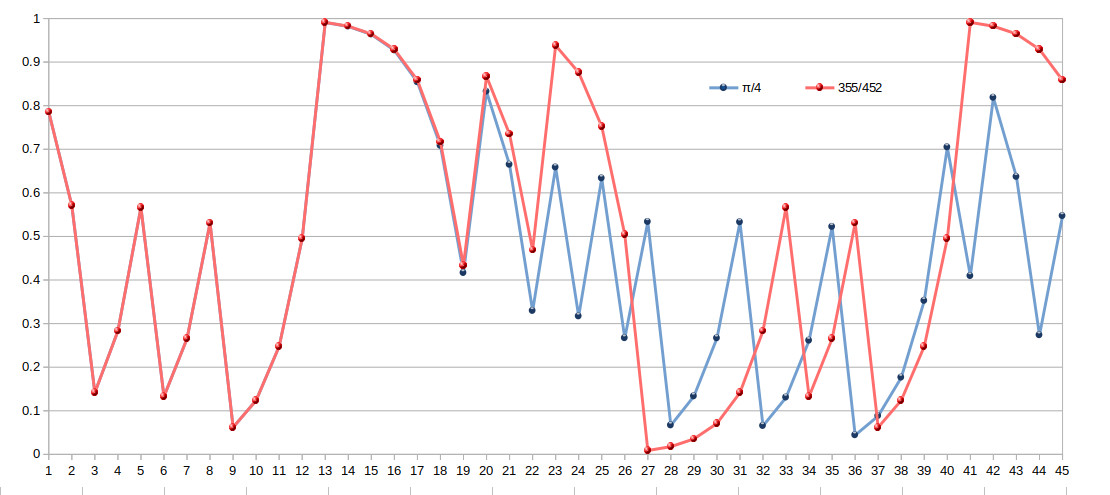
\includegraphics[scale=1.33]{img/comparaison.png}
\end{frame}
\begin{frame}
  \frametitle{décalage de Bernoulli : problème de \definecolor{rouge}{rgb}{0.8,0.2,0.2}
    précision}
  \begin{minipage}{0.49\textwidth}
    \definecolor{rouge}{rgb}{0.8,0.2,0.2}
    \begin{center}
      nombres réels \\
      précision limitée par la mémoire
    \end{center}
    \medskip
    \begin{tabular}{c c l}
      $\alpha_0$ & = & 0.1100100100001111110110 \\
      $\alpha_1$ & = & 0.100100100001111110110\textcolor{rouge}{0} \\
      $\alpha_2$ & = & 0.00100100001111110110\textcolor{rouge}{00} \\
      $\alpha_3$ & = & 0.0100100001111110110\textcolor{rouge}{000} \\
      \ldots \\
    \end{tabular} 
    \medskip
  \end{minipage}
  \onslide<2->{
    \begin{minipage}{0.49\textwidth}
      \definecolor{rouge}{rgb}{0.8,0.2,0.2}
      \begin{center}
        \textcolor{rouge}{\textbf{problème}} \\
        éviter la perte d'un bit \\
        à chaque étape \\
      \end{center}
      \medskip
    \end{minipage}}
  \onslide<3->{
    \begin{center}
      comment gérer des \\
      {\Large valeurs exactes\par} 
      pour $\alpha_n$ ? \\
    \end{center}}
\end{frame}
\subsection{Racines polynomiales de degré $3$}
\begin{frame}
  \frametitle{Racines polynomiales du degré 3}
  Solution de Saito et Yamaguchi (2017)\par\medskip
  $\alpha_n$  racine unique d’un polynôme du degré 3:  $f_n(\alpha_n) = 0$ \par
  avec $f_n(x) = x^3+b_n x^2+c_n x+d_n$. \par
  \onslide<2->{
    \medskip
    \begin{tabular}{*{6}{c}}
      où & $b_n^2-3 c_n \leqslant 0$
      & ; & $d_n < 0$
      & ; & $1 + b_n + c_n + d_n > 0$
    \end{tabular}}
  \onslide<3->{ 
    \par \medskip
    Exemple : $f_0(x) = x^3+x-1$\hfill{}$\epsilon_n = (\alpha_n)$\quad\phantom+\par
    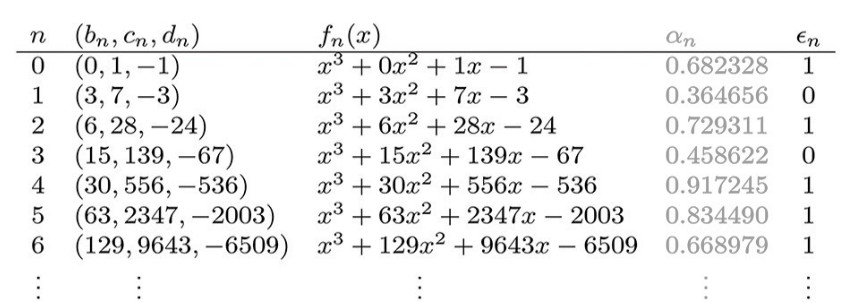
\includegraphics[scale=0.75]{img/SaitoYamaguchi2017.png}}
  \begin{center}
    \only<4>{\textbf{$\alpha_{n+1}=2 \alpha_n-\epsilon_n$ permet un calcul simple des coefficients de $f_{n+1}$} \\
      (opérations élémentaires)}
    \only<5>{$1 + 2b_n + 4c_n + 8d_n < 0 \ \Leftrightarrow \ \alpha_n > \frac{1}{2} \ \Leftrightarrow \ \epsilon_n = 1$ \\
      \textbf{évite le calcul des $\alpha_n$}}
    \only<6>{le stockage d'une seule étape demande beaucoup d'\textbf{espace mémoire}\\
      complexité en $O(n)$}
  \end{center}
\end{frame}
\ignore{
\subsection{Avantages/inconvénients de l'algorithme}
\begin{frame}
  \frametitle{Qualité du résultat et utilité de l'algorithme}
  \begin{center}
    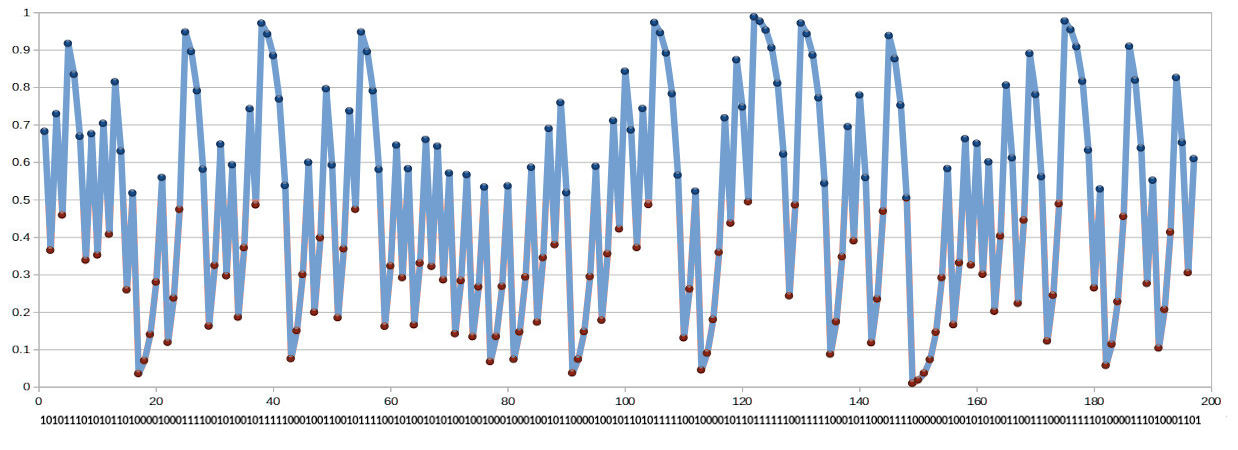
\includegraphics[scale=1]{img/graphique-chaos.png}\\
  \end{center}
  \begin{itemize}
  \item 
    calcul lent (pas de production on-the-fly)
  \item<2->  
    indépendance (imprévisibilité)
  \item<3->  
    avec un bon choix de $f_0$ ( $c_0$ assez grand et $d_0\geqslant-(b_0+c_0)$ ) \\
    distribution presque uniforme
  \item<4->
    bonne qualité $\rightarrow$ suites de test statistiques 
  \end{itemize} 
  \par \medskip
  \onslide<5>{
    \textbf{Référence} : 
    \textit{Pseudorandom number generator based on the Bernoulli map on cubic algebraic integers}, 
    Asaki Saito \& Akihiro Yamaguchi, 2017.} 
\end{frame}
}

\section{Générateurs de nombres ``vraiment'' aléatoires}
\minitoc
\subsection{Généralités - Processeur incapable}
\begin{frame}{Généralités - Processeur incapable}
\begin{itemize}
 \item Processeur arrive plutôt bien à propager de l’aléatoire
 \item Voir algorithmes présentés précédemment
 \item Mais il lui faut un coup de pouce au départ
 \item  Besoin d’une graine pour démarrer
 \item Pourquoi hasard inaccessible au processeur?
 \item Car le processeur est profondément déterministe
 \end{itemize}  
\end{frame}
\subsection{Algorithmes d'aggrégation et expansion d'entropie}
\begin{frame}{Algorithmes d'aggrégation et expansion d'entropie}
 \begin{itemize}
 \item Algorithme pour grossir le flux de TRNG (pas assez rapide)
 \item HAVEGE (utilisé par le noyau Linux)
 \item HArdware Volatile Entropy Gathering and Expansion
 \item https://www.irisa.fr/caps/projects/hipsor/misc.php
 \end{itemize}
\end{frame}
\subsection{Généralités - Le Monde réel oui}
\begin{frame}{Généralités - Le Monde réel oui}
 \begin{itemize}
 \item Aléatoire inévitable et dérangeant dans le monde réel!
   \begin{itemize}
   \item Incertitudes fondamentales des mesures
   \item Impossibilité de contrôler une valeur physique
   \end{itemize}
 \item Monde réel est donc LA source d’inspiration
 \end{itemize}
\end{frame}
\subsection{Collection d'entropie}
\begin{frame}{Collection d'entropie}
  \begin{itemize}
  \item Principales sources de hasard:
    \begin{itemize}
    \item phénomènes physiques stochastiques:
      \begin{itemize}
      \item bruit thermique (Johnson et Nyquist)
      \item autres phénomènes statistiques (vagues, etc.)
      \end{itemize}
    \item phénomènes quantiques intrinsèquement aléatoires
      \begin{itemize}
      \item effet photoélectrique
      \item n’importe quelle autre mesure quantique
      \end{itemize}
    \end{itemize}
  \end{itemize}
\end{frame}
\subsection{Le futur est-il quantique?}
\begin{frame}{Le futur est-il quantique?}
 \begin{itemize}
 \item Sources quantiques:
   \begin{itemize}
   \item source de radioactivité détectée par un compteur Geiger
   \item photons traversant un miroir semi-réfléchissant
   \item C’est le choix de la compagnie Genevoise ID Quantique
   \end{itemize}
 \end{itemize}
\end{frame}
\subsection{Exemple genevois: ID Quantique}
\begin{frame}{Exemple genevois: ID Quantique}
  \begin{itemize}
  \item Principe de la source ID Quantique:
    \begin{itemize}
    \item photons traversant un miroir semi-réfléchissant
    \item événements mutuellement exclusifs (réflexion / transmission)
    \item Détection associée respectivement à des valeurs de bit 0 ou 1
    \end{itemize}
  \end{itemize}
\end{frame}

\section{RNG dans Python}
\minitoc
\subsection{Que fait le module \textit{random} de Python?}
\begin{frame}
  \frametitle{Que fait le module ``random'' de Python?}
  \begin{itemize}
  \item<2-> Python fait appel à l'OS pour le TRNG.\par
    L'OS implémente typiquement un algorithme HAVEGE.
    \medskip
    \begin{itemize}
    \item utilisé directement par \texttt{random.SystemRandom} ou par
      \texttt{secrets}
      \par ce niveau d'aléatoire est nécessaire pour la cryptographie!
      \medskip
    \item utilisé en tant que \textit{seed} par défaut pour le PRNG de \texttt{random}
    \end{itemize}
    \bigskip
  \item<3-> Python utilise le \textbf{Mersenne Twister} en tant PRNG
    \begin{itemize}
    \item L'algorithme est plus complexe que ceux que nous avons présentés
      \medskip
    \item Il gère 624 nombres en parallèle, ce qui permet une période de
      $2^{19937}-1$, nettement plus que la limite naturelle de $2^{32}$.
    \end{itemize}
  \end{itemize}
\end{frame}
\ignore{
\begin{frame}[containsverbatim]{Que fait le module ``random'' de Python?}
  Le module \texttt{random} fournit des fonctions transformant directement ces
  nombres pour émuler des distributions aléatoires usuelles, le tirage sans
  remise, etc.
  \bigskip
  
\begin{lstlisting}
import random

# entier aléatoire entre 0 et 9
n = random.randrange(10)

# flottant aléatoire entre 0 et 10
x = random.uniform(0, 10)

# tirage de 2 éléments au hasard d'une liste
l = random.sample(["a", "b", "c", "d", "e"], 2)
\end{lstlisting}
\end{frame}
}
\subsection{Est-ce que ça marche?}
\begin{frame}{Est-ce que ça marche?}
  Tirage de 8000 nombres avec différents générateurs:
  %\vspace{-3ex}
  \begin{center}
    \begin{tikzpicture}
      % gestion d'étiquettage d'images selon la source suivante:
      % https://latexdraw.com/how-to-annotate-an-image-in-latex/
      \node[above right, inner sep=0] (image) at (0, 0) {
        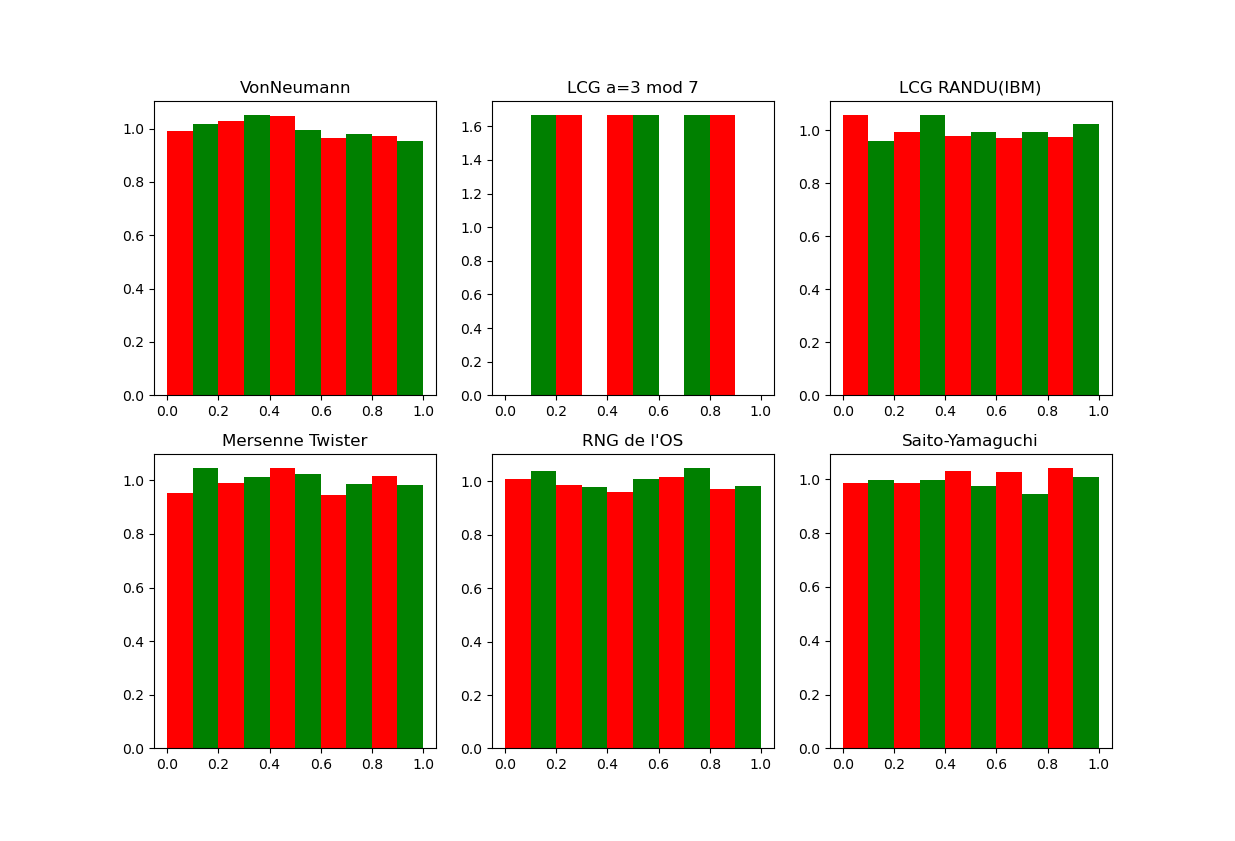
\includegraphics[width=0.8\textwidth]{img/rng8000b.png}
      };
      \begin{scope}[ % travailler "dans l'image"
        x={($0.1*(image.south east)$)},
        y={($0.1*(image.north west)$)}]
        % grille temporaire pour trouver où mettre les chi carrés
        %\draw[lightgray,step=1] (image.south west) grid (image.north east);
        %\foreach \x in {0,1,...,10} { \node [below] at (\x,0) {\x}; }
        %\foreach \y in {0,1,...,10} { \node [left] at (0,\y) {\y};}
        % et enfin les chi carrés
        \onslide<2->{
        \small\color{blue}\bfseries
        \node at (2.5, 7) {$\chi^2 = 8.4$};
        \node at (5, 7) {$\chi^2 = 5333$};
        \node at (8, 7) {$\chi^2 = 8.8$};
        \node at (2.5, 3) {$\chi^2 = 8.9$};
        \node at (5, 3) {$\chi^2 = 4.4$};
        \node at (8, 3) {$\chi^2 = 5.9$};
        }
      \end{scope}
    \end{tikzpicture}
  \end{center}
  code source: dossier \texttt{Code} dans \url{github.com/dalker/ASD2_RNG/}
\end{frame}
\ignore{
\subsection{Est-ce que ça marche?}
\begin{frame}{Est-ce que ça marche?}
  Tirages aléatoires avec \texttt{random.uniform(0, 1)} à partir d'une même
  seed.
  \vspace{-3ex}
  \begin{center}
    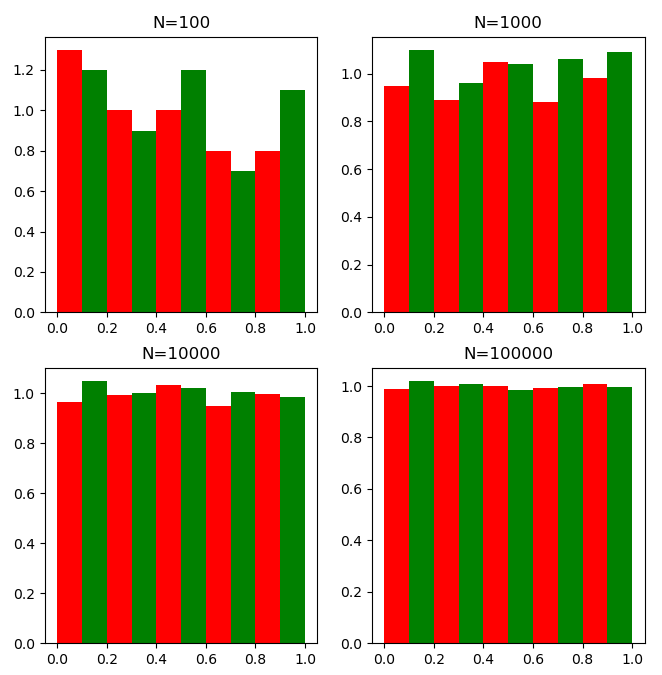
\includegraphics[width=0.5\textwidth]{img/uniformes.png}
  \end{center}
  code source: dossier \texttt{Code} dans \url{github.com/dalker/ASD2_RNG/}
\end{frame}
}
\begin{frame}{FIN}
  \begin{center}
    %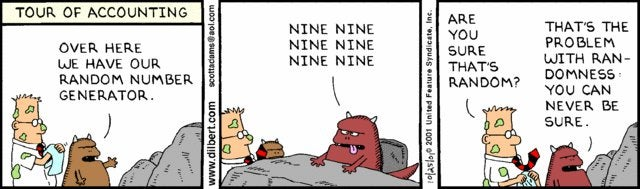
\includegraphics[width=.7\textwidth]{img/dilbert_evil.png}
    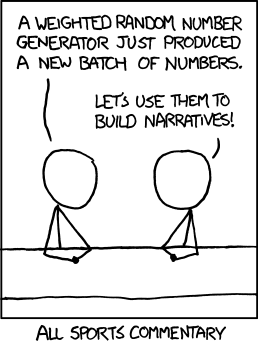
\includegraphics[width=.35\textwidth]{img/xkcd_sports.png}
  \end{center}
\end{frame}

\ignore{ % par le temps, on devra zapper - mais on garde le code ici si jamais
\begin{frame}
  \frametitle{Distributions aléatoires discrètes}
  \begin{itemize}
  \item $f(x)$, la ``fréquence'' de $x$, est la probabilité de tirer $x$.
  \item $f(x)\geq0, \;\forall x$
  \item $\sum_xf(x)=1$
  \end{itemize}
  \begin{tabular}{ccc}
    \onslide<2->{
    \begin{tikzpicture}[scale=.5, every node/.style={scale=0.5}]
      \draw[->] (-.2,0) -- (5.5,0) node[right] {$x$};
      \draw[->] (0, -0.2) -- (0, 4.2) node[above] {$f(x)$};
      \foreach \i in {1, ..., 5} {
        \draw[blue] (\i, 0) -- (\i, 3.5);
        \node at (\i, -0.3) {$\i$};
      }
      \draw (.1, 3.5) -- (-.1, 3.5) node[left] {$0.2$};
    \end{tikzpicture}}
    &\onslide<3->{
      \begin{tikzpicture}[scale=.5, every node/.style={scale=0.5}]
        \draw[->] (-1.2,0) -- (5.2,0) node[right] {$x$};
        \draw[->] (-1,-0.2) -- (-1,6.2) node[above] {$f(x)$};
        \draw[blue] (0, 0) -- (0, 1);
        \draw[blue] (1, 0) -- (1, 4);
        \draw[blue] (2, 0) -- (2, 6);
        \draw[blue] (3, 0) -- (3, 4);
        \draw[blue] (4, 0) -- (4, 1);
        \foreach \i in {0, ..., 5} {
          \node[below] at (\i, 0) {$\i$};
        }
      \end{tikzpicture}}
    &\onslide<4->{
      \begin{tikzpicture}[scale=.5, every node/.style={scale=0.5}]
        \draw[->] (-1.2,0) -- (4.2,0) node[right] {$x$};
        \draw[->] (-1,-0.2) -- (-1,4.2) node[above] {$f(x)$};
        \node[blue] at (1.5, 2) {\Huge ?};
      \end{tikzpicture}}
    \\
    \onslide<2->{uniforme} & \onslide<3->{binômiale} & \onslide<4->{autre}
  \end{tabular}    
\end{frame}
\begin{frame}
  \frametitle{Distributions aléatoires continues}
  \begin{itemize}
  \item $\int_a^bf(x)$ est la probabilité de tirer $x$ entre $a$ et $b$.
  %\item $f(x)\geq0, \;\forall x$
  \item $\int_{-\infty}^{+\infty}f(x)=1$
  \end{itemize}
  \begin{tikzpicture}
    \draw[->] (-.2,0) -- (4.2,0) node[right] {$x$};
    \draw[->] (0,-0.2) -- (0,2.2) node[above] {$f(x)$};
    \draw[blue] (1, 0) -- (1, 1) -- (3, 1) -- (3, 0);
    \draw (1, .1) -- (1, -.1) node[below] {\small$c$};
    \draw (3, .1) -- (3, -.1) node[below] {\small$d$};
    \node at (2, 2.2) {uniforme};
    \onslide<2->{
    \def\dx{6.8}; \def\dy{-3};
    \draw[->] (-4.2+\dx, \dy) -- (4.2+\dx,\dy) node[right] {$x$};
    \draw[->] (\dx-1,\dy-.2) -- (\dx-1, 2.2+\dy) node[above] {$f(x)$};
    \draw[blue] (\dx, \dy) plot[domain=-4:4, samples=200] ({\x+\dx},{\dy+2*2^(-\x*\x)});
    \draw (\dx, .1+\dy) -- (\dx, \dy-.1) node[below] {\small$\mu$};
    \def\ec{1.3}
    \draw (\dx+\ec, .1+\dy) -- (\dx+\ec, \dy-.1) node[below] {\small$\mu+\sigma$};
    \draw (\dx-\ec, .1+\dy) -- (\dx-\ec, \dy-.1) node[below] {\small$\mu-\sigma$};
    \node at (\dx+1, \dy+2.3) {normale};
    }\onslide<3->{
    \def\dx{8}; \def\dy{.5};
    \draw[->] (\dx-.2, \dy) -- (\dx+3.2,\dy) node[right] {$x$};
    \draw[->] (\dx-.1,\dy-.2) -- (\dx-.1, \dy+2.2) node[above] {$f(x)$};
    \node[blue] at (\dx+1.5, \dy+1) {\Huge ?};
    \node at (\dx+1.5, \dy+2.2) {autre};
    }
  \end{tikzpicture}
\end{frame}
}
\end{document}
